\documentclass{standalone}

\usepackage[american]{circuitikz}

\begin{document}
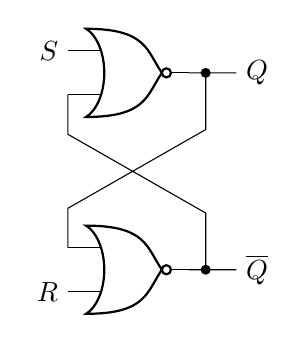
\begin{tikzpicture} \draw
	(0,0) node[nor port] (n1) {}
	(0,-2.5) node[nor port] (n2) {}
	
	(n1.in 1) node[left] {$S$}
	(n1.out) to [short] ++(0.6,0) node[right] {$Q$}
	
	(n2.in 2) node[left] {$R$}
	(n2.out) to [short] ++(0.6,0) node[right] {$\overline{Q}$}
	
	(n1.in 2) to [short] ++(0, -0.5) to [short] ++(1.75,-1) to [short, -*] ++(0, -0.72)
	(n2.in 1) to [short] ++(0, 0.5) to [short] ++(1.75,1) to [short, -*] ++(0, 0.72)
	;
\end{tikzpicture}
\end{document}